\section{Begriffe}

Eine \begriff{Sequenz} sind einzelne Anweisungen hintereinander. \\
Eine \begriff{Selektion} ist eine Verzweigung. \\
Eine \begriff{Repetition} ist eine Wiederholung.

\subsection{Variablen und Daten}

Wir sehen uns einen Biertrinker an, der nach dem Genuss noch ein paar Besorgungen machen muss. Dabei ergeben sich folgende Variablen
\begin{itemize}
	\item Variable \textbf{Durst} von Typ \textit{LOGICAL}
	\item Variable \textbf{Geld} von Typ \textit{INTEGER}
	\item Variable \textbf{PreisDerBesorgung} von Typ \textit{INTEGER}
	\item Variable \textbf{Rest} von Typ \textit{INTEGER}
	\item Variable \textbf{Bierpreis} von Typ \textit{INTEGER}
	\item Variable \textbf{WirtschaftAnnehmbar} von Typ \textit{LOGICAL}
	\item Variable \textbf{Autofahrer} von Typ \textit{LOGICAL}
	\item Variable \textbf{AlkoholGrenzwert} von Typ \textit{REAL}
	\item Variable \textbf{AlkoholVergiftungsWert} von Typ \textit{REAL}
\end{itemize}

\subsection{Schleifen}

In Fortran gibt es 4 Arten von \begriff{Schleifen}:
\begin{itemize}
	\item Endlosschleife
	\item Schleife mit Anfangsbedingung
	\item Schleife mit Endbedingung
	\item Zählschleife
\end{itemize}

Bei einer \begriff[Schleifen!]{Endlosschleife} wird der Anweisungsblock innerhalb der Schleife unendlich lange ausgeführt:
\begin{lstlisting}
do
 Anweisung1
 Anweisung2
 Anweisung3
end do
\end{lstlisting}

Bei einer \begriff[Schleifen!]{Schleife mit Anfangsbedingung} wird der Anweisungsblock nur ausgeführt, wenn die Anfangsbedingung wahr ist. Ist sie wahr, so wird der Block ausgeführt und anschließend überprüft, ob die Anfangsbedingung wieder wahr ist. Ist die Anfangsbedingung nicht wahr, so wird die Schleife nicht ausgeführt.
\begin{lstlisting}
do while(Anfangsbedingung)
 Anweisung1
 Anweisung2
 Anweisung3
end do
\end{lstlisting}

Hat die \begriff[Schleifen!]{Schleife eine Endbedingung}, so wird der Anweisungsblock auf jedem Fall 1-mal ausgeführt. Erst dann wird überprüft, ob die Endbedingung wahr ist. Ist sie das, wird die Schleife \textbf{verlassen}. Ist sie falsch, so wird die Schleife erneut ausgeführt.
\begin{lstlisting}
do
 Anweisung1
 Anweisung2
 Anweisung3
 if(Endbedingung) exit
end do
\end{lstlisting}

Eine \begriff[Schleifen!]{Zählschleife} in Fortran ist ähnlich wie in anderen Programmiersprachen konzipiert, aber die Syntax ist deutlich verschieden. Eine Zählschleife besitzt eine Zählvariable (die auch in der Schleife benutzt werden kann, aber nicht geändert werden sollte), die von einer Anfangszahl mit bestimmter Schrittweite solange hochgezählt (oder bei negativer Schrittweite heruntergezählt) wird, bis die Zählvariable die Endzahl erreicht.
\begin{lstlisting}
do i = anfang, ende, schrittweite
 Anweisung1
 Anweisung2
 Anweisung3
end do
\end{lstlisting}

Bitte beachten:
\begin{itemize}
	\item Der Zustand der Zählvariable \texttt{i} vor der Schleife geht verloren, auch wenn die Schleife 0-mal läuft.
	\item Die Zählvariable \texttt{i} darf im Inneren der Schleife nicht geändert werden.
	\item Der Endzustand der Zählvariable \texttt{i} ist nach der Schleife nicht definiert.
	\item Ausdrücke werden zu Beginn genau 1-mal (vor der ersten Iteration) berechnet und sind dann fest.
	\item Die Anzahl der Iterationen ist: $N=\max\left\lbrace 0,\texttt{nint}\left(\frac{\texttt{ende }-\texttt{ anfang }+\texttt{ i}}{\texttt{i}}\right)\right\rbrace$
\end{itemize}

\section{Einfache Syntax}

Es gibt einen zulässigen Fortran-Zeichensatz. Dieser umfasst zum Beispiel die Buchstaben A-Z und a-z, sowie 0-9, Sonderzeichen und Operatoren.

Nun einige lexikalische Einheiten (Symbole/Tokens):
\begin{itemize}
	\item Keywords sind nicht reserviert, Variablen können also auch nach Keywords benannt werden.
	\item Identifiers (Namen) haben eine Länge von maximal 63 Zeichen. Variablen können Buchstaben, Zahlen und auch den Unterstrich enthalten.
	\item Literale (Konstanten): 3 $\Rightarrow$ INTEGER, 2.876 $\Rightarrow$ REAL, .TRUE. $\Rightarrow$ LOGICAL, "'Hallo"' $\Rightarrow$ STRING
	\item Labels (Marken): 00000 ... 99999 sind Sprungmarken, die mit \texttt{GOTO 99999} erreicht werden können.
	\item Separatoren (Trennsymbole) sind: \texttt{()}, \texttt{/}, \texttt{/(/)}, \texttt{[]}, \texttt{=}, \texttt{=>}, \texttt{:}, \texttt{::}, \texttt{,}, \texttt{;} und \texttt{\%}.
	\item Operatoren sind: \texttt{+}, \texttt{-}, \texttt{*},\texttt{/}, \texttt{**}, \texttt{//}, \texttt{==}, \texttt{<=}, \texttt{<}, \texttt{/=}, \texttt{>}, \texttt{>=}, \texttt{.NOT.}, \texttt{.OR.}, \texttt{.AND.}, \texttt{.EQV.} und \texttt{.NEQV.}.
\end{itemize}

In den alten Quellformen bis vor Fortran-90, also insbesondere Fortran-66 und Fortran-77 waren
\begin{itemize}
	\item Namen maximal 6 Zeichen lang und
	\item Lochkarten 80 Zeichen breit.
\end{itemize}

\begin{center}
	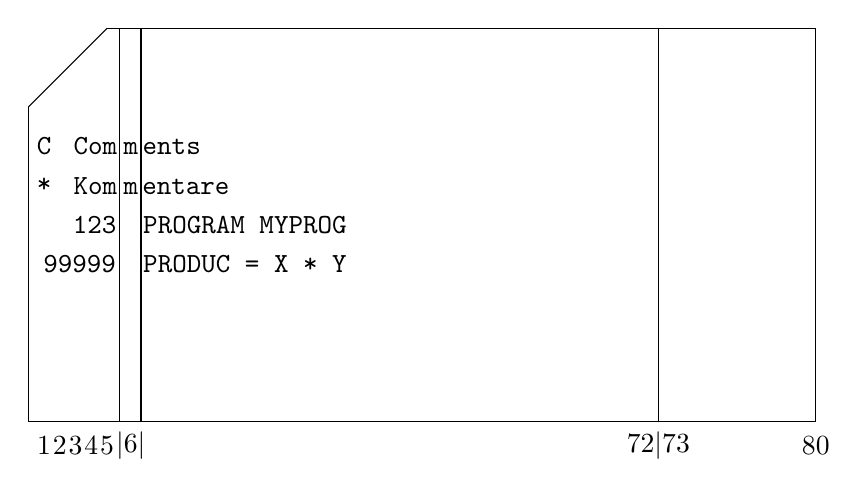
\begin{tikzpicture}
		\draw (0,0) -- (10,0);
		\draw (0,0) -- (0,4);
		\draw (0,4) -- (1,5);
		\draw (1,5) -- (10,5);
		\draw (10,0) -- (10,5);
		
		\node at (10,-0.3) (ende) {80};
		\node at (8,-0.3) (mitte) {$72\vert73$};
		\node at (0.2,-0.3) (1) {1};
		\node at (0.4,-0.3) (2) {2};
		\node at (0.6,-0.3) (3) {3};
		\node at (0.8,-0.3) (4) {4};
		\node at (1,-0.3) (5) {5};
		\node at (1.3,-0.3) (6) {$\vert 6\vert$};
		
		\draw (1.16,0) -- (1.16,5);
		\draw (1.43,0) -- (1.43,5);
		\draw (8,0) -- (8,5);
		
		\node at (0.2,3.5) (c) {\texttt{C}};
		\node at (0.85,3.5) (Com) {\texttt{Com}};
		\node at (1.3,3.47) (m) {\texttt{m}};
		\node at (1.82,3.488) (ents) {\texttt{ents}};
		
		\node at (0.2,3) (stern) {\texttt{*}};
		\node at (0.85,3) (Kom) {\texttt{Kom}};
		\node at (1.3,2.97) (m2) {\texttt{m}};
		\node at (2,2.99) (entare) {\texttt{entare}};
		
		\node at (0.84,2.5) (123) {\texttt{123}};
		\node at (2.75,2.5) (myprog) {\texttt{PROGRAM MYPROG}};
		\node at (0.65,2) (99999) {\texttt{99999}};
		\node at (2.75,2) (product) {\texttt{PRODUC = X * Y}};
	\end{tikzpicture}
\end{center}

Ab Fortran-90 wurden neue Quellformen entwickelt, das heißt:
\begin{itemize}
	\item Zeilen sind nun maximal 132 Zeichen lang
	\item Kommentare beginnen mit "'!"' und gehen bis zum Zeilenende
	\item Eine neue Zeile ist eine neue Anweisung, außer die letzte Zeile endet mit "'\&"'
	\item "'\&"' am Zeilenende bedeutet, dass die nächste nicht-Kommentar und nicht-Leerezeile die Anweisung fortsetzt.
	\item Die Fortsetzung darf mit "'\&"' beginnen.
	\item Es sind maximal 39 Fortsaetzungszeilen möglich
	\item Leerzeichen sind signifkant $\Rightarrow$ alle lexikalischen Tokens sind am Stück zu schreiben.
	\item Groß- und Kleinschreibung ist nicht signifikant in Namen und Keywords
\end{itemize}